%----------------------------------------------------------------------------------------
%	PACKAGES AND OTHER DOCUMENT CONFIGURATIONS
%----------------------------------------------------------------------------------------
\documentclass[11pt,a4paper]{article}

\usepackage[utf8]{inputenc} % to encode the document so that we can use more caracters (like Latin ones)
\usepackage[T1]{fontenc} % to encode the document so that we can use more caracters (like Latin ones)
\usepackage[english]{babel} % to write in English

\usepackage{geometry} % the paper's format and marges
\geometry{hmargin=2.3cm,vmargin=1.7cm}

\usepackage{titling} % to put the title where I want

% maths packages
\usepackage{mathtools}
\usepackage{amsmath,amsbsy,amsthm}
\usepackage{bm}
\usepackage{bigints}
\usepackage{stmaryrd}
\usepackage{amsfonts}

% graphs packages
\usepackage{graphicx}
\usepackage{float}
\usepackage{caption}
\usepackage{subcaption}
\usepackage{wrapfig,epsfig}

\usepackage{color}

\newtheorem{theorem}{Theorem}[section]
\newtheorem{lemma}[theorem]{Lemma}
\newtheorem{proposition}[theorem]{Proposition}
\newtheorem{corollary}[theorem]{Corollary}
\newtheorem{hypothese}[theorem]{Hypothesis}



\usepackage[final]{pdfpages}

\usepackage{algorithm}
\usepackage{algorithmic}
%----------------------------------------------------------------------------------------
%DOCUMENT
%----------------------------------------------------------------------------------------

\begin{document}
\newcommand{\intO}{\int_{\Omega}}
\newcommand{\intpO}{\int_{\partial\Omega}}
\newcommand{\bigintO}{\bigint_{\Omega}}
\newcommand{\bigintpO}{\bigint_{\partial\Omega}}

\newcommand{\intOi}[1]{\int_{\Omega_{#1}}}
\newcommand{\intpOi}[1]{\int_{\partial\Omega_{#1}}}
\newcommand{\bigintOi}[1]{\bigint_{\Omega_{#1}}}
\newcommand{\bigintpOi}[1]{\bigint_{\partial\Omega_{#1}}}

\newcommand{\dive}{\textrm{div}}
\newcommand{\acc}[1]{\left\{#1\right.}
\newcommand{\accTun}[1]{\left\{\begin{array}{l}#1\end{array}\right.}

\newcommand{\dist}{\textrm{dist}\,}
\newcommand{\tol}[1]{\textrm{tol}_{\textrm{#1}}}




\title{	Contrainte de circularité "par composantes connexes" (c.c.) }
\date{\today}

\maketitle


\section{Objectif du projet}

L'objectif ici est d'imposer a chaque composante connexe de la forme résultante d'avoir des sections circulaires. Ainsi, lors du processus couche par couche, chaque composante connexe d'une couche de la section devra "ressembler" à un cercle.

\section{Décomposition en composantes connexes}

L'algorithme de décomposition en composantes connexes est fait sous python de la manière suivante : 

\begin{itemize}
	\item Caractérisation des éléments solides : on définit une fonction qui donne les éléments qui sont solides ou non. Si la fonction levelset d'un des sommets de l'élément est négative, on considère l'élément complètement dans le solide.
	\item Caractérisation des voisins d'un élément : si l'élément est à côté est dans le même "état" (solide ou vide), il est considéré comme un voisin.
	\item Si deux éléments sont voisins, on leur attribue un parent commun et ainsi, on sépare les différentes composantes connexes.
\end{itemize}


\section{2 dimensions}

\subsection{Contrainte de circularité}

\subsubsection{Théorie}

En reprenant ce qui a été fait précédemment , on a une nouvelle fonction objectif sur le volume $\Omega \subset \mathbb{R}^2$. On note $NC(\Omega)$ le nombre de composantes connexes du volume $\Omega$ et, $forall i\in\llbracket 1, NC(\Omega) \rrbracket$, $\delta_{\Omega,i}(x)$ resprésente la fonction caractéristique de la composante connexe $i$. On a alors 

\begin{equation}
J(\Omega)=\sum_{i}^{NC(\Omega)}\intpOi{i} \dist(\Omega,i,s)^2ds=\sum_{i}^{NC(\Omega)}\intpO \delta_{\Omega,i}(s)\dist(\Omega,i,s)^2ds
\end{equation}

avec 

\begin{equation}
\dist(\Omega,i,s)=\sqrt{\left(X(s)-\frac{\intO \delta_{\Omega,i}(x)X(x)dx}{\intO \delta_{\Omega,i}(x)dx}\right)^2+\left(Y(s)-\frac{\intO \delta_{\Omega,i}(x)Y(x)dx}{\intO \delta_{\Omega,i}(x)dx}\right)^2}-\sqrt{\frac{\intO \delta_{\Omega,i}(x)dx}{\pi}}
\end{equation}

Afin de simplifier le problème, on réalise une première hypothèse :

\begin{hypothese}
	\label{hyp:H1}
	$NC(\Omega)=NC$, on suppose que le nombre de composantes connexes ne dépend pas de $\Omega$ (et donc pas besoin de le dériver).
\end{hypothese}


On a alors $J(\Omega)=\sum_{i}^{NC}\intpO \delta_{\Omega,i}(s)\dist(\Omega,i,s)^2ds$ et, en dérivant par rapport à $\Omega$,

\begin{equation}
\begin{array}{l}
J'(\Omega)(\theta)=\intO 2\dist(\Omega,i,s)\delta_{\Omega,i}(s)\dist '(\Omega,i,s)(\theta)ds+\intO \dist(\Omega,i,s)^2\delta_{\Omega,i}'(s)(\theta)ds\\
\\
\, +\sum_{i}^{NC}\intpO \left[\frac{\partial \delta_{\Omega,i}(s)}{\partial n}\dist(\Omega,i,s)^2+2\dist(\Omega,i,s)\delta_{\Omega,i}(s)\frac{\partial\dist(\Omega,i,s)}{\partial n}+H(s)\dist(\Omega,i,s)^2\delta_{\Omega,i}(s)\right]\theta(s)n(s)ds
\end{array}
\end{equation}

\begin{hypothese}
	\label{hyp:H2}
	On néglige les dérivées de $\delta_{\Omega,i}(s)$ que ce soit de forme ou le gradient.
\end{hypothese}

En notant $\dist(\Omega,i,s)=\dist(s)$ et en définissant comme suit les fonctions suivante :

\begin{equation}
\begin{array}{ll}
A(\Omega,i)=\intOi{i}dx=\intO \delta_{\Omega,i}(x)dx; & \, \\
\\
Cx(\Omega,i)=\intOi{i}X(x)dx=\intO X(x)\delta_{\Omega,i}(x)dx; & Cy(\Omega,i)=\intOi{i}Y(x)dx=\intO Y(x)\delta_{\Omega,i}(x)dx;\\	
\\
Dx(\Omega,i,x)=X(x)-\frac{Cx(\Omega,i)}{A(\Omega,i)} =Dx(i,x);& Dy(\Omega,i,x)=Y(x)-\frac{Cy(\Omega,i)}{A(\Omega,i)}=Dy(i,x); \\
\\
DE(\Omega,i,x)=Dx(\Omega,i,x)^2+Dy(\Omega,i,x)^2; &\dist(\Omega,i,s)=\dist(i,s) \\
\\
A_1(\Omega,i)=\intpOi{i}\frac{2\dist(i,s')Dx(i,s')}{\sqrt{DE(\Omega,i,s')}A(\Omega,i)} ds'=A_1(i) & A_2(\Omega,i)=\intpOi{i}\frac{2\dist(i,s')Dy(i,s')}{\sqrt{DE(\Omega,i,s')}A(\Omega,i)}ds'=A_2(i) \\
\\
A_3(\Omega,i)=\intpOi{i}\frac{\dist(i,s')}{\sqrt{A(\Omega,i)\pi}}ds'=A_3(i) 
\end{array}
\end{equation}

on a le théorème suivant.

\begin{theorem}
	Avec les notations définies précédemment et sous les hypothèses \ref{hyp:H1} et \ref{hyp:H2}, on a 
	\begin{equation}
	J'(\Omega)(\theta)=\sum_{i}^{NC}\intpOi{i}\left[2\textrm{\dist}(i,s)\frac{\partial\textrm{\dist}(i,s)}{\partial n}+H(s)\textrm{\dist}(i,s)^2-A_1Dx(i,s)-A_2Dy(i,s)-A_3\right]\theta(s)n(s)ds
	\end{equation}
\end{theorem}


\begin{proof}
	En utilisant les hypothèses \ref{hyp:H1} et \ref{hyp:H2}, on a 
	\begin{equation}
	\begin{array}{l}
	J'(\Omega)(\theta)=\sum_{i}^{NC}\intpO \left[\overbrace{\frac{\partial \delta_{\Omega,i}(s)}{\partial n}\dist(\Omega,i,s)^2}^\text{\textrm{neglige}}+2\dist(i,s)\delta_{\Omega,i}(s)\frac{\partial\dist(i,s)}{\partial n}+H(s)\dist(i,s)^2\delta_{\Omega,i}(s)\right]\theta(s)n(s)ds\\
	\quad +\intO 2\dist(i,s)\delta_{\Omega,i}(s)\dist '(i,s)(\theta)ds+\underbrace{\intO \dist(i,s)^2\delta_{\Omega,i}'(s)(\theta)ds}_\text{\textrm{neglige}}\\
	\end{array}
	\end{equation}
	
	et donc :
	
	\begin{equation}
	\begin{array}{ll}
	J'(\Omega)(\theta)=&\sum_{i}^{NC}\intpO \left[2\dist(i,s)\delta_{\Omega,i}(s)\frac{\partial\dist(i,s)}{\partial n}+H(s)\dist(i,s)^2\delta_{\Omega,i}(s)\right]\theta(s)n(s)ds\\
	\\
	\, & +\intO 2\dist(i,s)\delta_{\Omega,i}(s)\dist '(i,s)(\theta)ds
	\end{array}
	\end{equation}
	
	En continuant à négliger les dérivées de la caractéristique de la composante connexe, on a aussi :
	
	\begin{equation}
	\begin{array}{l}
		A'(\Omega,i)(\theta)=\intpO \delta_{\Omega,i}(s)\theta(s)n(s)ds+\overbrace{\intO \delta_{\Omega,i}'(x)(\theta)dx}^\text{neglige}= \intpO \delta_{\Omega,i}(s)\theta(s)n(s)ds\\
		\\
		Cx'(\Omega,i)(\theta)=\intpO \delta_{\Omega,i}(s)X(s)\theta(s)n(s)ds+\overbrace{\intO X(x)\delta_{\Omega,i}'(x)(\theta)dx}^\text{neglige}= \intpO X(s)\delta_{\Omega,i}(s)\theta(s)n(s)ds\\
		\\
		Cy'(\Omega,i)(\theta)=\intpO \delta_{\Omega,i}(s)Y(s)\theta(s)n(s)ds+\overbrace{\intO Y(x)\delta_{\Omega,i}'(x)(\theta)dx}^\text{neglige}= \intpO Y(s)\delta_{\Omega,i}(s)\theta(s)n(s)ds\\
	\end{array}
	\end{equation}
	
	d'où
	
	\begin{equation}
	\begin{array}{l}
		Dx'(i,x)(\theta)=\frac{-1}{A(\Omega,i)}\intpO\delta_{\Omega,i}(s)Dx(i,s)\theta(s)n(s)ds\\
		\\
		Dy'(i,x)(\theta)=\frac{-1}{A(\Omega,i)}\intpO\delta_{\Omega,i}(s)Dy(i,s)\theta(s)n(s)ds\\
	\end{array}
	\end{equation}
	
	Cela donne donc :
	
	\begin{equation}
	\begin{array}{ll}
	J'(\Omega)(\theta)=\sum_{i}^{NC}\Bigg[\bigintpO\bigg[ &\delta_{\Omega,i}(s)\left(2\dist(i,s)\frac{\partial\dist(i,s)}{\partial n}+H(s)\dist(i,s)^2\right)\theta(s)n(s)\\
	\\
	\,&-\overbrace{\intpO \delta_{\Omega,i}(s')\frac{2\dist(i,s')Dx(i,s')}{\sqrt{DE(\Omega,i,s')}A(\Omega,i)}ds'}^\text{A1} Dx(i,s)\delta_{\Omega,i}(s)\theta(s)n(s) \\
	\\
	\, & -\overbrace{\intpO \delta_{\Omega,i}(s')\frac{2\dist(i,s')Dy(i,s')}{\sqrt{DE(\Omega,i,s')}A(\Omega,i)}ds'}^\text{A2} Dy(i,s)\delta_{\Omega,i}(s)\theta(s)n(s)\\
	\\
	\, & -\overbrace{\intpO \delta_{\Omega,i}(s')\frac{\dist(i,s')}{\sqrt{A(\Omega,i)\pi}}ds'}^\text{A3} \delta_{\Omega,i}(s) \theta(s)n(s)\bigg]ds \Bigg]
	\end{array}
	\end{equation}
	 d'où le résultat.
\end{proof}



La régularisation du problème entraîne $NC$ problêmes variationnels du type : trouver $Q_i$ tel que pour tout $W\in H^1(D)$,

\begin{equation}
\begin{array}{l}
\int_D \alpha^2\nabla Q_i\nabla W+Q_iW=\\
\qquad\intpOi{i}\left[2\textrm{dist}(i,s)\frac{\partial\textrm{dist}(i,s)}{\partial n}+H(s)\textrm{dist}(i,s)^2-A_1(i)Dx(i,s)-A_2(i)Dy(i,s)-A_3(i)\right]Wds
\end{array}
\end{equation}

On a alors une vitesse d'advection par composante connexe : $vh_i=-Q_i$ et la vitesse d'advection totale est $vh=\sum_i^{NC}vh_i$


\subsubsection{Gestion du cercle sur le bord}
Dans le cas précédent, la manière de gérer le fait le domaine $\Omega$ puisse couper les bords du domaine de calcul est la suivante :
\begin{itemize}
	\item on "modifie" la fonction level set $\phi$ du domaine afin que tout le solide soit représenté à l'intérieur du domaine. Pour cela, on résout un problème variationnel afin que 
	\begin{equation}
	\accTun{
		\forall x\in D \setminus (\partial D\cup\partial\Omega), \phi_{modifie}(x)=\phi(x) \\
		\\
		\forall x\in\partial D\cup\partial\Omega, \phi_{modifie}(x)=0
		}
	\end{equation}
	
	\item on calcule ensuite la fonction objectif de circularité. Ainsi, une composante connexe qui coupait le bord verra l'intégralité de sa frontière compter, même la partie qui était préalablement sur le bord du domaine de calcul.
	\item le cercle correspondant va couper le bord du domaine. Ceci est accepté et l'algorithme va chercher à pousser la composante connexe vers ce cercle dont une partie est "fictive". La forme résultante sur le domaine de calcul sera un cercle coupé. 
	
	\item l'optimum de la fonction objectif ne sera pas 0 mais on pourra alors considérer que la forme est optimale.
\end{itemize}

D'autres choix de modélisation pourraient être adoptés. Par exemple :
\begin{itemize}
	\item on pourrait décider de calculer la distance du centre du cercle au bord du domaine de calcul. Si le rayon du cercle est supérieur à cette distance, cela signifie que le cercle va couper le bord du domaine. On prend alors pour cercle approximateur le cercle trouvé précédemment translaté dans la direction qui avait permis de trouver la distance du centre du cercle au bord du domaine de calcul, d'un facteur faisant que le bord du cercle se retrouve au bord du domaine de calcul (facteur rayon-distance du centre). Le calcul de la fonction objectif se fait alors avec ce cercle approximateur. Il faut cependant dériver cette modification par rapport à la à la forme $\Omega$.

\end{itemize}

\subsubsection{Gestion des changements de topologie}
On remarque qu'un changement de topologie telle qu'une fusion de deux composantes connexes ou la division de l'une d'elle en deux distinctes entraine une discontinuité de la fonction objectif et doit donc être gérer dans l'algorithme d'optimisation afin que la descente de gradient ne se bloque pas. Plusieurs possibilités sont ici possibles :

\begin{itemize}
	\item On accepte automatiquement l'itération s'il y a eu changement de topologie.
	\item On adapte une fonction de tolérance qui permet certains changements de topologie et en empèche d'autres. 
\end{itemize}

On a choisi pour le cas en deux dimensions d'utiliser la première solution.

\subsubsection{Remarque de modélisation}
On note que la gestion ici de la contrainte de cercle impacte le résultat. En effet, si une composante connexe du solide n'est pas convexe (trou au milieu en particulier), la modélisation choisie va tendre à remplir ce vide afin d'obtenir un vrai cercle. Les tubes ne pourront être modélisés par cette méthode.

\subsubsection{Algorithme de résolution}
 voir le code
 

\subsubsection{Résultats}
\paragraph{Initialisation 1}

\vspace{0cm}

On considère l'initialisation présentée en Figure \ref{fig:Ini1-1}. Le résultat, après 20 itérations, est présenté en Figure \ref{fig:Ini1-2}. La variation de la fonction objectif en fonction des itérations est présentée en Figure \ref{fig:Ini1-3}.

\begin{figure}[H]
	\begin{minipage}{0.33\textwidth}
		\centering
		\includegraphics[width=0.6\textwidth]{/Users/mathilde/These/Projets/FormeSection/SectionCercle/CercleCompConnexe/2D/ContrainteSeule/AccepteChangementTopo/SansPousserBord/ResultatsTests/ellipse/it1}
		\label{fig:Ini1-1}
	\end{minipage}
	\begin{minipage}{0.33\textwidth}
		\centering
		\includegraphics[width=0.6\textwidth]{/Users/mathilde/These/Projets/FormeSection/SectionCercle/CercleCompConnexe/2D/ContrainteSeule/AccepteChangementTopo/SansPousserBord/ResultatsTests/ellipse/it20}
		\label{fig:Ini1-2}
	\end{minipage}
	\begin{minipage}{0.33\textwidth}
		\centering
		\includegraphics[width=\textwidth]{/Users/mathilde/These/Projets/FormeSection/SectionCercle/CercleCompConnexe/2D/ContrainteSeule/AccepteChangementTopo/SansPousserBord/ResultatsTests/ellipse/contrainte.png}
		\label{fig:Ini1-3}
	\end{minipage}
\end{figure}


\paragraph{Initialisation 2}

\vspace{0cm}

On considère l'initialisation présentée en Figure \ref{fig:Ini3-1}. Le résultat, après 20 itérations, est présenté en Figure \ref{fig:Ini3-2}. La variation de la fonction objectif en fonction des itérations est présentée en Figure \ref{fig:Ini3-3}. On constate bien pic dans la fonction objectif au moment de fusion entre les deux composantes connexes.

\begin{figure}[H]
	\begin{minipage}{0.33\textwidth}
		\centering
		\includegraphics[width=0.6\textwidth]{/Users/mathilde/These/Projets/FormeSection/SectionCercle/CercleCompConnexe/2D/ContrainteSeule/AccepteChangementTopo/SansPousserBord/ResultatsTests/SymBridge14/it1}
		\label{fig:Ini3-1}
	\end{minipage}
	\begin{minipage}{0.33\textwidth}
		\centering
		\includegraphics[width=0.6\textwidth]{/Users/mathilde/These/Projets/FormeSection/SectionCercle/CercleCompConnexe/2D/ContrainteSeule/AccepteChangementTopo/SansPousserBord/ResultatsTests/SymBridge14/it30}
		\label{fig:Ini3-2}
	\end{minipage}
	\begin{minipage}{0.33\textwidth}
		\centering
		\includegraphics[width=\textwidth]{/Users/mathilde/These/Projets/FormeSection/SectionCercle/CercleCompConnexe/2D/ContrainteSeule/AccepteChangementTopo/SansPousserBord/ResultatsTests/SymBridge14/contrainte.png}
		\label{fig:Ini3-3}
	\end{minipage}
\end{figure}


\paragraph{Initialisation 3}

\vspace{0cm}

On considère l'initialisation présentée en Figure \ref{fig:Ini2-1}. Le résultat, après 20 itérations, est présenté en Figure \ref{fig:Ini2-2}. La variation de la fonction objectif en fonction des itérations est présentée en Figure \ref{fig:Ini2-3}. On constate bien pic dans la fonction objectif au moment de fusion entre les deux composantes connexes.

\begin{figure}[H]
	\begin{minipage}{0.33\textwidth}
		\centering
		\includegraphics[width=0.6\textwidth]{/Users/mathilde/These/Projets/FormeSection/SectionCercle/CercleCompConnexe/2D/ContrainteSeule/AccepteChangementTopo/SansPousserBord/ResultatsTests/MoitiePleinUnTrou/it1}
		\label{fig:Ini2-1}
	\end{minipage}
	\begin{minipage}{0.33\textwidth}
		\centering
		\includegraphics[width=0.6\textwidth]{/Users/mathilde/These/Projets/FormeSection/SectionCercle/CercleCompConnexe/2D/ContrainteSeule/AccepteChangementTopo/SansPousserBord/ResultatsTests/MoitiePleinUnTrou/it30}
		\label{fig:Ini2-2}
	\end{minipage}
	\begin{minipage}{0.33\textwidth}
		\centering
		\includegraphics[width=\textwidth]{/Users/mathilde/These/Projets/FormeSection/SectionCercle/CercleCompConnexe/2D/ContrainteSeule/AccepteChangementTopo/SansPousserBord/ResultatsTests/MoitiePleinUnTrou/contrainte.png}
		\label{fig:Ini2-3}
	\end{minipage}
\end{figure}


\subsection{Ajout d'une contrainte de volume}

\subsubsection{Contrainte de volume}
On ajoute à la fonction objectif de circularité précédente une contrainte de volume : le volume global de la section doit rester constant, c'est-à-dire que :

\begin{equation}
\intO dx=\intOi{0}dx=V_0
\end{equation}

On a donc une contrainte du type 

\begin{equation}
C(\Omega)=\left(\intO dx-V_0\right)^2-\tol{cont}
\end{equation}

On peut calculer la vitesse d'advection liée à la contrainte en résolvant un problème de régularisation et en prenant $vh_{vol}=-Q$:

\begin{equation}
\int_D \alpha^2 \nabla Q\nabla W +QWdx=\intpO 2\left(\intO dx-V_0\right)Wds
\end{equation}

\subsubsection{Gestion de la contrainte}
En utilisant un multiplicateur de Lagrange fixe, on a la fonction Lagrangienne suivante :
\begin{equation}
L(\Omega)=J(\Omega)=\sum_{i}^{NC(\Omega)}\intpOi{i} \dist(\Omega,i,s)^2ds+l_{vol}C(\Omega)
\end{equation}

et on prend pour vitesse d'advection (en utilisant le même facteur $\alpha$ dans tous les problèmes de régularisation) 
\begin{equation}
vh=\sum_i^{NC}vh_{cercle,i}+l_{vol}vh_{vol}
\end{equation}

et on met à jour le multiplicateur de Lagrange de la manière suivante :

\begin{equation}
\accTun{
	l_{vol}=0 \qquad \qquad  \qquad \qquad \textrm{si\,} C(\Omega)\leq 0\\
	\\
	l_{vol}=l_{vol}+\textrm{step}_{vol}C(\Omega) \quad \textrm{sinon}	
	}
\end{equation}

\subsubsection{Résultats}

On reprend les initialisations précédentes pour tester cette partie.  On choisit ici pour tolérance 1\% du volume de départ pour l'initialisation 1 et 10\% pour les deux suivantes. Ce choix est arbitraire et peut être adapté. En l'occurence ici, avec ces choix là, on n'a pas de variation de volume.

\paragraph{Initialisation 1}

\vspace{0cm}

On considère l'initialisation présentée en Figure \ref{fig:2DVIni1-1}. Le résultat, après 20 itérations, est présenté en Figure \ref{fig:2DVIni1-2}. La variation de la fonction objectif en fonction des itérations est présentée en Figure \ref{fig:2DVIni1-3} et celle du volume en Figure \ref{fig:2DVIni1-4}.

\begin{figure}[H]
	\begin{minipage}{0.48\textwidth}
		\centering
		\includegraphics[width=0.6\textwidth]{/Users/mathilde/These/Projets/FormeSection/SectionCercle/CercleCompConnexe/2D/ContrainteVolume/AccepteChangementTopo/SansPousserBord/ResultatsTests/ellipse/it1}
		\label{fig:2DVIni1-1}
	\end{minipage}
	\begin{minipage}{0.48\textwidth}
		\centering
		\includegraphics[width=0.6\textwidth]{/Users/mathilde/These/Projets/FormeSection/SectionCercle/CercleCompConnexe/2D/ContrainteVolume/AccepteChangementTopo/SansPousserBord/ResultatsTests/ellipse/it20}
		\label{fig:2DVIni1-2}
	\end{minipage}	
\end{figure}

\begin{figure}[H]
		\begin{minipage}{0.48\textwidth}
			\centering
			\includegraphics[width=\textwidth]{/Users/mathilde/These/Projets/FormeSection/SectionCercle/CercleCompConnexe/2D/ContrainteVolume/AccepteChangementTopo/SansPousserBord/ResultatsTests/ellipse/contrainte.png}
			\label{fig:2DVIni1-3}
		\end{minipage}
		\begin{minipage}{0.48\textwidth}
			\centering
			\includegraphics[width=\textwidth]{/Users/mathilde/These/Projets/FormeSection/SectionCercle/CercleCompConnexe/2D/ContrainteVolume/AccepteChangementTopo/SansPousserBord/ResultatsTests/ellipse/volCont.png}
			\label{fig:2DVIni1-4}
		\end{minipage}
\end{figure}


\paragraph{Initialisation 2}

\vspace{0cm}

On considère l'initialisation présentée en Figure \ref{fig:2DVIni2-1}. Le résultat, après 20 itérations, est présenté en Figure \ref{fig:2DVIni-2}. La variation de la fonction objectif en fonction des itérations est présentée en Figure \ref{fig:2DVIni2-3} et celle de volume en Figure \ref{fig:2DVIni2-4}. On constate bien pic dans la fonction objectif au moment de fusion entre les deux composantes connexes.

\begin{figure}[H]
	\begin{minipage}{0.48\textwidth}
		\centering
		\includegraphics[width=0.6\textwidth]{/Users/mathilde/These/Projets/FormeSection/SectionCercle/CercleCompConnexe/2D/ContrainteVolume/AccepteChangementTopo/SansPousserBord/ResultatsTests/SymBridge14/it1}
		\label{fig:2DVIni2-1}
	\end{minipage}
	\begin{minipage}{0.48\textwidth}
		\centering
		\includegraphics[width=0.6\textwidth]{/Users/mathilde/These/Projets/FormeSection/SectionCercle/CercleCompConnexe/2D/ContrainteVolume/AccepteChangementTopo/SansPousserBord/ResultatsTests/SymBridge14/it30}
		\label{fig:2DVIni2-2}
	\end{minipage}
\end{figure}

\begin{figure}[H]
	\begin{minipage}{0.48\textwidth}
		\centering
		\includegraphics[width=\textwidth]{/Users/mathilde/These/Projets/FormeSection/SectionCercle/CercleCompConnexe/2D/ContrainteVolume/AccepteChangementTopo/SansPousserBord/ResultatsTests/SymBridge14/contrainte.png}
		\label{fig:2DVIni2-3}
	\end{minipage}
	\begin{minipage}{0.48\textwidth}
		\centering
		\includegraphics[width=\textwidth]{/Users/mathilde/These/Projets/FormeSection/SectionCercle/CercleCompConnexe/2D/ContrainteVolume/AccepteChangementTopo/SansPousserBord/ResultatsTests/SymBridge14/volCont.png}
		\label{fig:2DVIni2-4}
	\end{minipage}
\end{figure}

\paragraph{Initialisation 3}

\vspace{0cm}

On considère l'initialisation présentée en Figure \ref{fig:2DVIni3-1}. Le résultat, après 20 itérations, est présenté en Figure \ref{fig:2DVIni3-2}. La variation de la fonction objectif en fonction des itérations est présentée en Figure \ref{fig:2DVIni3-3} et celle du volume en Figure \ref{fig:2DVIni3-4}. On constate bien pic dans la fonction objectif au moment de fusion entre les deux composantes connexes.

\begin{figure}[H]
	\begin{minipage}{0.48\textwidth}
		\centering
		\includegraphics[width=0.6\textwidth]{/Users/mathilde/These/Projets/FormeSection/SectionCercle/CercleCompConnexe/2D/ContrainteVolume/AccepteChangementTopo/SansPousserBord/ResultatsTests/MoitiePleinUnTrou/it1}
		\label{fig:2DVIni3-1}
	\end{minipage}
	\begin{minipage}{0.48\textwidth}
		\centering
		\includegraphics[width=0.6\textwidth]{/Users/mathilde/These/Projets/FormeSection/SectionCercle/CercleCompConnexe/2D/ContrainteVolume/AccepteChangementTopo/SansPousserBord/ResultatsTests/MoitiePleinUnTrou/it30}
		\label{fig:2DVIni3-2}
	\end{minipage}
\end{figure}

\begin{figure}[H]
	\begin{minipage}{0.48\textwidth}
		\centering
		\includegraphics[width=\textwidth]{/Users/mathilde/These/Projets/FormeSection/SectionCercle/CercleCompConnexe/2D/ContrainteVolume/AccepteChangementTopo/SansPousserBord/ResultatsTests/MoitiePleinUnTrou/contrainte.png}
		\label{fig:2DVIni3-3}
	\end{minipage}
	\begin{minipage}{0.48\textwidth}
		\centering
		\includegraphics[width=\textwidth]{/Users/mathilde/These/Projets/FormeSection/SectionCercle/CercleCompConnexe/2D/ContrainteVolume/AccepteChangementTopo/SansPousserBord/ResultatsTests/MoitiePleinUnTrou/volCont.png}
		\label{fig:2DVIni3-4}
	\end{minipage}
\end{figure}




\section{3 dimensions}

\subsection{Contrainte de circularité}

\subsubsection{Theorie}

On considère maintenant un volume $\Omega$ en trois dimensions. Il modélise un solide construit couche par couche, de direction privilégiée $(Oz)$. On cherche a optimiser chaque section plane du solide d'équation $(z=h)$ afin que chaque composante connexe du solide sur cette section soit circulaire. En notant $H$ la hauteur totale du solide, $dh$ l'épaisseur d'une couche et $N_{couche}$ le nombre de couches, on a donc la fonction objectif suivante :

\begin{equation}
J(\Omega)=\int_0^H \sum_{i}^{NC(\Omega,h)}\intpOi{i} \dist(\Omega,i,h,s)^2dsdh=\int_0^H\sum_{i}^{NC(\Omega,h)}\intpO \delta_{\Omega,i}(s)\delta_{z=h}(s)\dist(\Omega,i,h,s)^2dsdh
\end{equation}
 
On applique ici aussi l'hypothèse \ref{hyp:H1} et on peut donc simplifier la fonction objectif :

\begin{equation}
J(\Omega)=\int_0^H \sum_{i}^{NC(h)}\intpOi{i} \dist(\Omega,i,h,s)^2dsdh=\int_0^H\sum_{i}^{NC(h)}\intpO \delta_{\Omega,i}(s)\delta_{z=h}(s)\dist(\Omega,i,h,s)^2dsdh
\end{equation}

On pose une nouvelle hypothèse  afin de déterminer la dérivée de forme de cette fonction objectif.

\begin{hypothese}
	\label{hyp:H3}
	On néglige $\frac{\partial \delta_{z=h}(s)}{\partial n}$. 
\end{hypothese}

En notant $\dist(\Omega,i,s)=\dist(s)$ et en définissant comme suit les fonctions suivante :

\begin{equation}
\begin{array}{ll}
A(\Omega,i,h)=\intOi{i}dx=\intO \delta_{z=h}(x)\delta_{\Omega,i}(x)dx; & \, \\
\\
Cx(\Omega,i,h)=\intOi{i}X(x)dx=\intO X(x)\delta_{z=h}(x)\delta_{\Omega,i}(x)dx; & Cy(\Omega,i,h)=\intOi{i}Y(x)dx=\intO Y(x)\delta_{z=h}(x)\delta_{\Omega,i}(x)dx;\\	
\\
Dx(\Omega,i,h,x)=X(x)-\frac{Cx(\Omega,i,h)}{A(\Omega,i,h)} =Dx(i,h,x);& Dy(\Omega,i,h,x)=Y(x)-\frac{Cy(\Omega,i,h)}{A(\Omega,i,h)}=Dy(i,h,x); \\
\\
DE(\Omega,i,h,x)=Dx(\Omega,i,h,x)^2+Dy(\Omega,i,h,x)^2; &\dist(\Omega,i,h,s)=\dist(i,h,s) \\
\\
A_1(\Omega,i,h)=\intpOi{i}\frac{2\dist(i,h,s')Dx(i,s')}{\sqrt{DE(\Omega,i,h,s')}A(\Omega,i,h)} ds'=A_1(i,h)=A_1 & A_2(\Omega,i,h)=\intpOi{i}\frac{2\dist(i,h,s')Dy(i,s')}{\sqrt{DE(\Omega,i,h,s')}A(\Omega,i,h)}ds'=A_2(i,h)=A_2 \\
\\
A_3(\Omega,i,h)=\intpOi{i}\frac{\dist(i,h,s')}{\sqrt{A(\Omega,i,h)\pi}}ds'=A_3(i,h)=A_3 
\end{array}
\end{equation}

on a le théorème suivant.

\begin{theorem}
	Avec les notations définies précédemment et sous les hypothèses \ref{hyp:H1} et \ref{hyp:H2}, on a 
	\begin{equation}
\begin{array}{l}
	J'(\Omega)(\theta)= \\
	 \int_0^H\sum_{i}^{NC(h)}\intpOi{i}\left[2\textrm{\dist}(i,h,s)\frac{\partial\textrm{\dist}(i,h,s)}{\partial n}+H(s)\textrm{\dist}(i,h,s)^2-A_1Dx(i,h,s)-A_2Dy(i,h,s)-A_3\right]\theta(s)n(s)dsdh
\end{array}
	\end{equation}
\end{theorem}

\begin{proof}
	En utilisant les hypothèses \ref{hyp:H1}, \ref{hyp:H2} et \ref{hyp:H3}, on a ($\delta_{z=h}$ est indépendent de $\Omega$)
	\begin{equation}
	\begin{array}{l}
	J'(\Omega)(\theta)=\int_0^H\sum_{i}^{NC(h)}\Bigg[ 	\bigintpO \overbrace{\left(\frac{\partial \delta_{\Omega,i}(s)}{\partial n}\delta_{z=h}(s)+\frac{\partial \delta_{z=h}(s)}{\partial n}\delta_{\Omega,i}(s)\right)\dist(\Omega,i,s)^2}^\text{\textrm{neglige}}\theta(s)n(s)ds \\
	\qquad \qquad \qquad \quad +\bigintpO \left[2\dist(i,s)\delta_{\Omega,i}(s)\delta_{z=h}(s)\frac{\partial\dist(i,s)}{\partial n}+H(s)\dist(i,s)^2\delta_{\Omega,i}(s)\delta_{z=h}(s)\right]\theta(s)n(s)ds\\
	\qquad \qquad \qquad \quad +\bigintO 2\dist(i,s)\delta_{\Omega,i}(s)\delta_{z=h}(s)\dist '(i,s)(\theta)ds+\underbrace{\intO \dist(i,s)^2\delta_{z=h}(s)\delta_{\Omega,i}'(s)(\theta)ds}_\text{\textrm{neglige}}\Bigg]\\
	\end{array}
	\end{equation}
	
	Or, comme précédemment, on a 
	
	\begin{equation}
	\begin{array}{ll}
	A'(\Omega,i,h)(\theta)= \intpO \delta_{\Omega,i}(s)\delta_{z=h}(s)\theta(s)n(s)ds &\, \\
	\\
	Cx'(\Omega,i)(\theta)=\intpO X(s)\delta_{z=h}(s)\delta_{\Omega,i}(s)\theta(s)n(s)ds; & Cy'(\Omega,i)(\theta)= \intpO Y(s)\delta_{z=h}(s)\delta_{\Omega,i}(s)\theta(s)n(s)ds\\
	\end{array}
	\end{equation}
	
	d'où
	
	\begin{equation}
	\begin{array}{l}
	Dx'(i,h,x)(\theta)=\frac{-1}{A(\Omega,i,h)}\intpO\delta_{\Omega,i}(s)\delta_{z=h}(s)Dx(i,h,s)\theta(s)n(s)ds\\
	\\
	Dy'(i,h,x)(\theta)=\frac{-1}{A(\Omega,i,h)}\intpO\delta_{\Omega,i}(s)\delta_{z=h}(s)Dy(i,h,s)\theta(s)n(s)ds\\
	\end{array}
	\end{equation}
	
	Cela donne donc :
	
	\begin{equation}
	\begin{array}{ll}
	J'(\Omega)(\theta)=\bigint_0^H&\sum_{i}^{NC(h)}\Bigg[\bigintpO\bigg[ \delta_{z=h}(s)\delta_{\Omega,i}(s)\left(2\dist(i,h,s)\frac{\partial\dist(i,h,s)}{\partial n}+H(s)\dist(i,h,s)^2\right)\theta(s)n(s)\\
	\\
	\,&-\overbrace{\intpO \delta_{z=h}(s')\delta_{\Omega,i}(s')\frac{2\dist(i,h,s')Dx(i,h,s')}{\sqrt{DE(\Omega,i,h,s')}A(\Omega,i,h)}ds'}^\text{A1} Dx(i,h,s)\delta_{z=h}(s)\delta_{\Omega,i}(s)\theta(s)n(s) \\
	\\
	\, & -\overbrace{\intpO \delta_{z=h}(s')\delta_{\Omega,i}(s')\frac{2\dist(i,h,s')Dy(i,h,s')}{\sqrt{DE(\Omega,i,h,s')}A(\Omega,i,h)}ds'}^\text{A2} Dy(i,h,s)\delta_{z=h}(s)\delta_{\Omega,i}(s)\theta(s)n(s)\\
	\\
	\, & -\overbrace{\intpO \delta_{z=h}(s')\delta_{\Omega,i}(s')\frac{\dist(i,h,s')}{\sqrt{A(\Omega,i,h)\pi}}ds'}^\text{A3} \delta_{z=h}(s)\delta_{\Omega,i}(s)\theta(s)n(s)\bigg]ds \Bigg]dh
	\end{array}
	\end{equation}
\end{proof}	

	On discrétise ensuite en espace en calculant la contrainte sur chaque couche. 
	La dérivée de forme ne dépendant ici que de $x$ et $y$ et donc du plan $(z=h)$, on simplifie le problème de régularisation, Pour chaque composante connexe de chaque couche, on résout $NC(h)$ problèmes :
	
	\begin{equation}
	\begin{array}{l}
	\int_{D\cup (z=h)} \alpha^2\nabla Q_i\nabla W+Q_iWds=\\
	\qquad\intpOi{i}\left[2\textrm{dist}(i,h,s)\frac{\partial\textrm{dist}(i,h,s)}{\partial n}+H(s)\textrm{dist}(i,h,s)^2-A_1(i,h)Dx(i,h,s)-A_2(i,h)Dy(i,h,s)-A_3(i,h)\right]Wds
	\end{array}
	\end{equation}
	
	On obtient alors pour chaque composante connexe une velocité d'advection sur le plan, $v_h(h,i)$. On la multiplie par une fonction gaussienne en z centrée sur $z=h$ et "normalisée". On a alors pour chaque section une vitesse d'advection :
	
	\begin{equation}
	v_h(\Omega,z=h)=\sum_{i=1}^{i=NC(h)}\frac{v_h(h,i)*\exp(-100(z-h)^2)}{\int_D \exp(-100(z'-h)^2)dx'dy'dz'}
	\end{equation}
	
	Pour avoir la vitesse d'advection totale, il suffit ensuite de sommer sur le nombre de couches :
	
	\begin{equation}
	v_h(\Omega)=\sum_{couche=0}^{couche=N_{couche}}dh*v_h(\Omega,z=h_{couche})
	\end{equation}

\subsubsection{Gestion des cercles sur le bord}

La gestion des cercles sur les bords du domaine de calcul s'effectue de la même manière que dans le cas de la dimension 2. 

\subsubsection{Gestion des changements de topologie}
 Trois méthodes différentes ont été expérimentées :
 \begin{itemize}
 	\item Adaptation de la tolérance afin que les changements de topologies soient absorbés.
 	\item Acceptation de l'itération dès que l'une des sections subit un changement de topologie.
 	\item On n'inclue pas dans le calcul de la fonction objectif la section qui change de topologie (on garde son impact sur la vitesse d'advection cependant).
 \end{itemize}
 
\subsubsection{Algorithme}

\subsubsection{Résultats}

\paragraph{Adaptation de la tolérance}
On teste ici la première technique de gestion des changements de topologie.

\subparagraph{Initialisation 1} On utilise ici l'initialisation présentée dans la figure \ref{fig:cercleseul3Dini1}.

\begin{figure}[H]
	\label{fig:cercleseul3Dini1}
	\begin{minipage}{0.32\textwidth}
		\centering
		\includegraphics[width=0.8\textwidth]{/Users/mathilde/These/Projets/FormeSection/SectionCercle/CercleCompConnexe/3D/ContrainteSeule/SansPousserBord/Tolerance/ResultatsTests/Ini3/it1-1.png}
	\end{minipage}
	\begin{minipage}{0.32\textwidth}
		\centering
		\includegraphics[width=0.8\textwidth]{/Users/mathilde/These/Projets/FormeSection/SectionCercle/CercleCompConnexe/3D/ContrainteSeule/SansPousserBord/Tolerance/ResultatsTests/Ini3/it1-2.png}
	\end{minipage}
	\begin{minipage}{0.32\textwidth}
		\centering
		\includegraphics[width=0.8\textwidth]{/Users/mathilde/These/Projets/FormeSection/SectionCercle/CercleCompConnexe/3D/ContrainteSeule/SansPousserBord/Tolerance/ResultatsTests/Ini3/it1-3.png}
	\end{minipage}	
	\caption{Initialisation 1}	
\end{figure}

On obtient le résultat suivant (Figure \ref{fig:cercleseul3Dini1Fin}) après 98 itérations et la decroissance de la fonction objectif suivante:

\begin{figure}[H]
	\label{fig:cercleseul3Dini1Fin}
	\begin{minipage}{0.33\textwidth}
		\centering
		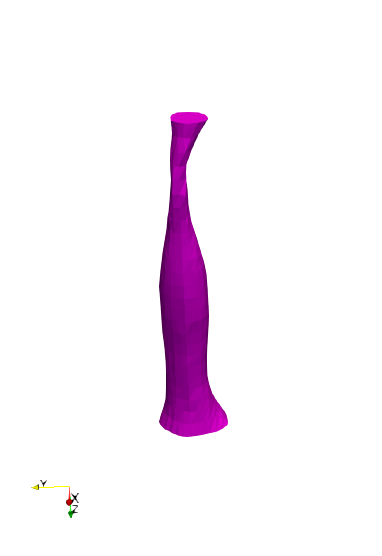
\includegraphics[width=0.8\textwidth]{/Users/mathilde/These/Projets/FormeSection/SectionCercle/CercleCompConnexe/3D/ContrainteSeule/SansPousserBord/Tolerance/ResultatsTests/Ini3/it98-1.png}
	\end{minipage}
	\begin{minipage}{0.33\textwidth}
		\centering
		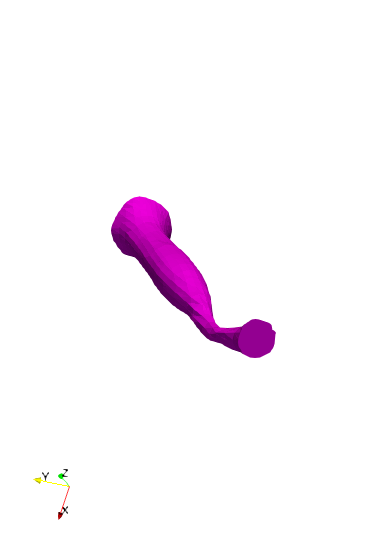
\includegraphics[width=0.8\textwidth]{/Users/mathilde/These/Projets/FormeSection/SectionCercle/CercleCompConnexe/3D/ContrainteSeule/SansPousserBord/Tolerance/ResultatsTests/Ini3/it98-2.png}
	\end{minipage}	
	\begin{minipage}{0.33\textwidth}
		\centering
		\includegraphics[width=0.8\textwidth]{/Users/mathilde/These/Projets/FormeSection/SectionCercle/CercleCompConnexe/3D/ContrainteSeule/SansPousserBord/Tolerance/ResultatsTests/Ini3/objF.png}
	\end{minipage}	
	\caption{Résultats de l'initialisation 1 et décroissance de la fonction objectif}	
\end{figure}

\subparagraph{Initialisation 2} On utilise ici l'initialisation présentée dans la figure \ref{fig:cercleseul3Dini2}.

\begin{figure}[H]
	\label{fig:cercleseul3Dini2}
	\begin{minipage}{0.45\textwidth}
		\centering
		\includegraphics[width=0.8\textwidth]{/Users/mathilde/These/Projets/FormeSection/SectionCercle/CercleCompConnexe/3D/ContrainteSeule/SansPousserBord/Tolerance/ResultatsTests/Ini2/it1-1.png}
	\end{minipage}
	\begin{minipage}{0.45\textwidth}
		\centering
		\includegraphics[width=0.8\textwidth]{/Users/mathilde/These/Projets/FormeSection/SectionCercle/CercleCompConnexe/3D/ContrainteSeule/SansPousserBord/Tolerance/ResultatsTests/Ini2/it1-2.png}
	\end{minipage}
	\caption{Initialisation 2}	
\end{figure}

On obtient le résultat suivant (Figure \ref{fig:cercleseul3Dini2Fin}) après 199 itérations et la decroissance de la fonction objectif suivante:

\begin{figure}[H]
	\label{fig:cercleseul3Dini2Fin}
	\begin{minipage}{0.33\textwidth}
		\centering
		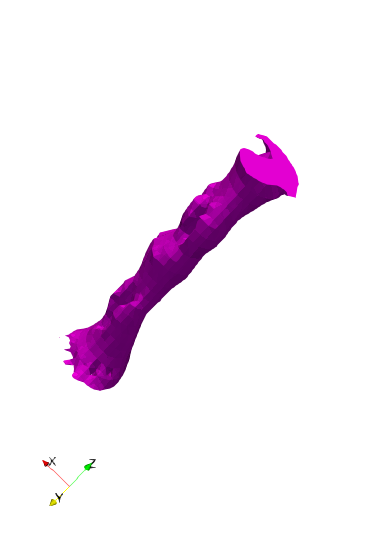
\includegraphics[width=0.8\textwidth]{/Users/mathilde/These/Projets/FormeSection/SectionCercle/CercleCompConnexe/3D/ContrainteSeule/SansPousserBord/Tolerance/ResultatsTests/Ini2/it199-1.png}
	\end{minipage}
	\begin{minipage}{0.33\textwidth}
		\centering
		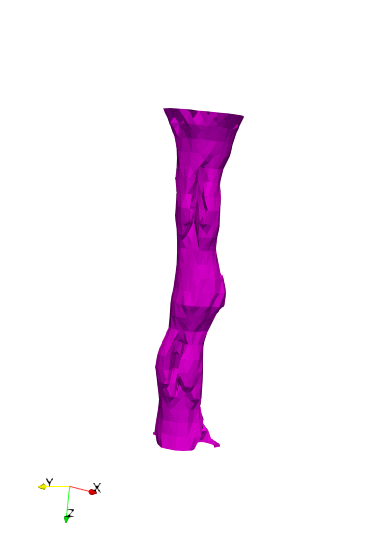
\includegraphics[width=0.8\textwidth]{/Users/mathilde/These/Projets/FormeSection/SectionCercle/CercleCompConnexe/3D/ContrainteSeule/SansPousserBord/Tolerance/ResultatsTests/Ini2/it199-2.png}
	\end{minipage}	
	\begin{minipage}{0.33\textwidth}
		\centering
		\includegraphics[width=0.8\textwidth]{/Users/mathilde/These/Projets/FormeSection/SectionCercle/CercleCompConnexe/3D/ContrainteSeule/SansPousserBord/Tolerance/ResultatsTests/Ini2/objF.png}
	\end{minipage}	
	\caption{Résultats de l'initialisation 2 et décroissance de la fonction objectif}	
\end{figure}


\subparagraph{Initialisation 3} On utilise ici l'initialisation présentée dans la figure \ref{fig:cercleseul3Dini3}.

\begin{figure}[H]
	\label{fig:cercleseul3Dini3}
	\begin{minipage}{0.32\textwidth}
		\centering
		\includegraphics[width=0.8\textwidth]{/Users/mathilde/These/Projets/FormeSection/SectionCercle/CercleCompConnexe/3D/ContrainteSeule/SansPousserBord/Tolerance/ResultatsTests/Ini4/it1-1.png}
	\end{minipage}
	\begin{minipage}{0.32\textwidth}
		\centering
		\includegraphics[width=0.8\textwidth]{/Users/mathilde/These/Projets/FormeSection/SectionCercle/CercleCompConnexe/3D/ContrainteSeule/SansPousserBord/Tolerance/ResultatsTests/Ini4/it1-2.png}
	\end{minipage}
	\begin{minipage}{0.32\textwidth}
		\centering
		\includegraphics[width=0.8\textwidth]{/Users/mathilde/These/Projets/FormeSection/SectionCercle/CercleCompConnexe/3D/ContrainteSeule/SansPousserBord/Tolerance/ResultatsTests/Ini4/it1-3.png}
	\end{minipage}	
	\caption{Initialisation 3}	
\end{figure}

On obtient le résultat suivant (Figure \ref{fig:cercleseul3Dini3Fin}) après 98 itérations et la decroissance de la fonction objectif suivante:

\begin{figure}[H]
	\label{fig:cercleseul3Dini3Fin}
	\begin{minipage}{0.45\textwidth}
		\centering
		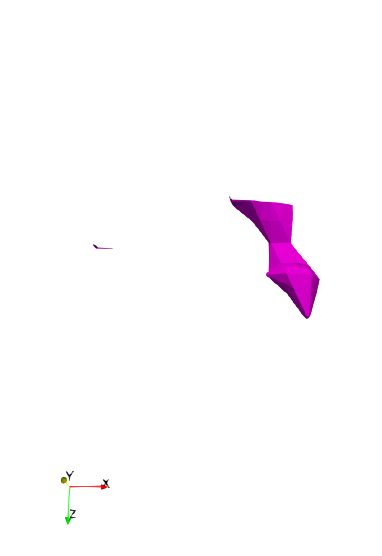
\includegraphics[width=0.8\textwidth]{/Users/mathilde/These/Projets/FormeSection/SectionCercle/CercleCompConnexe/3D/ContrainteSeule/SansPousserBord/Tolerance/ResultatsTests/Ini4/it199.png}
	\end{minipage}	
	\begin{minipage}{0.45\textwidth}
		\centering
		\includegraphics[width=0.8\textwidth]{/Users/mathilde/These/Projets/FormeSection/SectionCercle/CercleCompConnexe/3D/ContrainteSeule/SansPousserBord/Tolerance/ResultatsTests/Ini4/objF.png}
	\end{minipage}	
	\caption{Résultats de l'initialisation 3 et décroissance de la fonction objectif}	
\end{figure}



\paragraph{Acceptation de l'itération dès que l'une des sections change de topologie}
On teste ici la seconde technique de gestion des changements de topologie.


\subparagraph{Initialisation 1} On utilise ici l'initialisation présentée dans la figure \ref{fig:cercleseul3Daini1}.

\begin{figure}[H]
	\label{fig:cercleseul3Daini1}
	\begin{minipage}{0.32\textwidth}
		\centering
		\includegraphics[width=0.8\textwidth]{/Users/mathilde/These/Projets/FormeSection/SectionCercle/CercleCompConnexe/3D/ContrainteSeule/SansPousserBord/Tolerance/ResultatsTests/Ini3/it1-1.png}
	\end{minipage}
	\begin{minipage}{0.32\textwidth}
		\centering
		\includegraphics[width=0.8\textwidth]{/Users/mathilde/These/Projets/FormeSection/SectionCercle/CercleCompConnexe/3D/ContrainteSeule/SansPousserBord/Tolerance/ResultatsTests/Ini3/it1-2.png}
	\end{minipage}
	\begin{minipage}{0.32\textwidth}
		\centering
		\includegraphics[width=0.8\textwidth]{/Users/mathilde/These/Projets/FormeSection/SectionCercle/CercleCompConnexe/3D/ContrainteSeule/SansPousserBord/Tolerance/ResultatsTests/Ini3/it1-3.png}
	\end{minipage}	
	\caption{Initialisation 1}	
\end{figure}

On obtient le résultat suivant (Figure \ref{fig:cercleseul3Dsini1Fin}) après 119 itérations et la decroissance de la fonction objectif suivante:

\begin{figure}[H]
	\label{fig:cercleseul3Dsini1Fin}
	\begin{minipage}{0.33\textwidth}
		\centering
		\includegraphics[width=0.8\textwidth]{/Users/mathilde/These/Projets/FormeSection/SectionCercle/CercleCompConnexe/3D/ContrainteSeule/SansPousserBord/AccepteChangementTopo/ResultatsTests/Ini3/it119-1.png}
	\end{minipage}
	\begin{minipage}{0.33\textwidth}
		\centering
		\includegraphics[width=0.8\textwidth]{/Users/mathilde/These/Projets/FormeSection/SectionCercle/CercleCompConnexe/3D/ContrainteSeule/SansPousserBord/AccepteChangementTopo/ResultatsTests/Ini3/it119-2.png}
	\end{minipage}	
	\begin{minipage}{0.33\textwidth}
		\centering
		\includegraphics[width=0.8\textwidth]{/Users/mathilde/These/Projets/FormeSection/SectionCercle/CercleCompConnexe/3D/ContrainteSeule/SansPousserBord/AccepteChangementTopo/ResultatsTests/Ini3/objF.png}
	\end{minipage}	
	\caption{Résultats de l'initialisation 1 et décroissance de la fonction objectif}	
\end{figure}

\subparagraph{Initialisation 2} On utilise ici l'initialisation présentée dans la figure \ref{fig:cercleseul3Daini2}.

\begin{figure}[H]
	\label{fig:cercleseul3Daini2}
	\begin{minipage}{0.45\textwidth}
		\centering
		\includegraphics[width=0.8\textwidth]{/Users/mathilde/These/Projets/FormeSection/SectionCercle/CercleCompConnexe/3D/ContrainteSeule/SansPousserBord/Tolerance/ResultatsTests/Ini2/it1-1.png}
	\end{minipage}
	\begin{minipage}{0.45\textwidth}
		\centering
		\includegraphics[width=0.8\textwidth]{/Users/mathilde/These/Projets/FormeSection/SectionCercle/CercleCompConnexe/3D/ContrainteSeule/SansPousserBord/Tolerance/ResultatsTests/Ini2/it1-2.png}
	\end{minipage}
	\caption{Initialisation 2}	
\end{figure}

On obtient le résultat suivant (Figure \ref{fig:cercleseul3Daini2Fin}) après 119 itérations et la decroissance de la fonction objectif suivante:

\begin{figure}[H]
	\label{fig:cercleseul3Daini2Fin}
	\begin{minipage}{0.33\textwidth}
		\centering
		\includegraphics[width=0.8\textwidth]{/Users/mathilde/These/Projets/FormeSection/SectionCercle/CercleCompConnexe/3D/ContrainteSeule/SansPousserBord/AccepteChangementTopo/ResultatsTests/Ini2/it119-1.png}
	\end{minipage}
	\begin{minipage}{0.33\textwidth}
		\centering
		\includegraphics[width=0.8\textwidth]{/Users/mathilde/These/Projets/FormeSection/SectionCercle/CercleCompConnexe/3D/ContrainteSeule/SansPousserBord/AccepteChangementTopo/ResultatsTests/Ini2/it119-2.png}
	\end{minipage}	
	\begin{minipage}{0.33\textwidth}
		\centering
		\includegraphics[width=0.8\textwidth]{/Users/mathilde/These/Projets/FormeSection/SectionCercle/CercleCompConnexe/3D/ContrainteSeule/SansPousserBord/AccepteChangementTopo/ResultatsTests/Ini2/objF.png}
	\end{minipage}	
	\caption{Résultats de l'initialisation 2 et décroissance de la fonction objectif}	
\end{figure}


\subparagraph{Initialisation 3} On utilise ici l'initialisation présentée dans la figure \ref{fig:cercleseul3Daini3}.

\begin{figure}[H]
	\label{fig:cercleseul3Daini3}
	\begin{minipage}{0.32\textwidth}
		\centering
		\includegraphics[width=0.8\textwidth]{/Users/mathilde/These/Projets/FormeSection/SectionCercle/CercleCompConnexe/3D/ContrainteSeule/SansPousserBord/Tolerance/ResultatsTests/Ini4/it1-1.png}
	\end{minipage}
	\begin{minipage}{0.32\textwidth}
		\centering
		\includegraphics[width=0.8\textwidth]{/Users/mathilde/These/Projets/FormeSection/SectionCercle/CercleCompConnexe/3D/ContrainteSeule/SansPousserBord/Tolerance/ResultatsTests/Ini4/it1-2.png}
	\end{minipage}
	\begin{minipage}{0.32\textwidth}
		\centering
		\includegraphics[width=0.8\textwidth]{/Users/mathilde/These/Projets/FormeSection/SectionCercle/CercleCompConnexe/3D/ContrainteSeule/SansPousserBord/Tolerance/ResultatsTests/Ini4/it1-3.png}
	\end{minipage}	
	\caption{Initialisation 3}	
\end{figure}

On obtient le résultat suivant (Figure \ref{fig:cercleseul3Daini3Fin}) après 98 itérations et la decroissance de la fonction objectif suivante:

\begin{figure}[H]
	\label{fig:cercleseul3Daini3Fin}
	\begin{minipage}{0.45\textwidth}
		\centering
		\includegraphics[width=0.8\textwidth]{/Users/mathilde/These/Projets/FormeSection/SectionCercle/CercleCompConnexe/3D/ContrainteSeule/SansPousserBord/AccepteChangementTopo/ResultatsTests/Ini4/it119-1.png}
	\end{minipage}	
	\begin{minipage}{0.45\textwidth}
		\centering
		\includegraphics[width=0.8\textwidth]{/Users/mathilde/These/Projets/FormeSection/SectionCercle/CercleCompConnexe/3D/ContrainteSeule/SansPousserBord/AccepteChangementTopo/ResultatsTests/Ini4/objF.png}
	\end{minipage}	
	\caption{Résultats de l'initialisation 3 et décroissance de la fonction objectif}	
\end{figure}

\section{Optimisation de la circularité par c.c. avec contrainte de volume par section}

\subsection{Théorie}

On décide maintenant, de la même manière que dans le cas 2D, d'ajouter pour chaque section une contrainte de conservation de la surface. On conserve toutes les hypothèses déjà faites et on obtient une nouvelle fonction objectif :

\begin{equation}
\tilde{J}(\Omega)=J(\Omega)+l_{vol}*V(\Omega)=\int_0^H \sum_{i}^{NC(h)}\intpOi{i} \dist(\Omega,i,h,s)^2dsdh+l_{vol}*\int_0^H\sum_{i}^{NC(h)}\left(\intpOi{i}ds-V{cible,i}\right)^2-tol
\end{equation}

On garde donc la vitesse d'advection déjà déterminée et on ajoute une nouvelle vitesse liée au volume. En prenant la même partie bilinéaire del'équation de régularisation de la vitesse que précédemment, on a la linéarité sur le vitesse d'advection.

Pour chaque section, on résout donc un problème variationnel du type :

	\begin{equation}
	\int_{D\cup (z=h)} \alpha^2\nabla Q_i\nabla W+Q_iWds=\intpOi{i}grh_{vol,i}Wds
	\end{equation}

avec 

\begin{equation}
grh_{vol,i}=2\left(\intpOi{i}ds-V{cible,i}\right)
\end{equation}

La vitesse d'advection finale sera donc $v=v_{cercle}+l_{vol}v_{vol}$.

On a présenté ce résultat avec $l_{vol}$ non précisé. On utilise ici une méthode Lagrangienne. On initialise alors $l_{vol}$ à 0 et on le met à jour au fur et à mesure des itérations selon le schéma suivant :
\begin{equation}
\accTun{
	l_{vol}=0 \qquad \qquad  \qquad \qquad \textrm{si\,} V(\Omega)\leq 0\\
	\\
	l_{vol}=l_{vol}+\textrm{step}_{vol}V(\Omega) \quad \textrm{sinon}	
}
\end{equation}

La gestion des cercles sur le bord ainsi et les changements de topologie sont traités de la même manière que précédemment.

\subsection{Algorithme}

\subsection{Résultats}



\paragraph{Adaptation de la tolérance}
On teste ici la première technique de gestion des changements de topologie.

%\subparagraph{Initialisation 1} On utilise ici l'initialisation présentée dans la figure \ref{fig:cercleseul3Dini1}.
%
%\begin{figure}[H]
%	\label{fig:cercleseul3Dini1}
%	\begin{minipage}{0.32\textwidth}
%		\centering
%		\includegraphics[width=0.8\textwidth]{/Users/mathilde/These/Projets/FormeSection/SectionCercle/CercleCompConnexe/3D/ContrainteSeule/SansPousserBord/Tolerance/ResultatsTests/Ini3/it1-1.png}
%	\end{minipage}
%	\begin{minipage}{0.32\textwidth}
%		\centering
%		\includegraphics[width=0.8\textwidth]{/Users/mathilde/These/Projets/FormeSection/SectionCercle/CercleCompConnexe/3D/ContrainteSeule/SansPousserBord/Tolerance/ResultatsTests/Ini3/it1-2.png}
%	\end{minipage}
%	\begin{minipage}{0.32\textwidth}
%		\centering
%		\includegraphics[width=0.8\textwidth]{/Users/mathilde/These/Projets/FormeSection/SectionCercle/CercleCompConnexe/3D/ContrainteSeule/SansPousserBord/Tolerance/ResultatsTests/Ini3/it1-3.png}
%	\end{minipage}	
%	\caption{Initialisation 1}	
%\end{figure}
%
%On obtient le résultat suivant (Figure \ref{fig:cercleseul3Dini1Fin}) après 98 itérations et la decroissance de la fonction objectif suivante:
%
%\begin{figure}[H]
%	\label{fig:cercleseul3Dini1Fin}
%	\begin{minipage}{0.33\textwidth}
%		\centering
%		\includegraphics[width=0.8\textwidth]{/Users/mathilde/These/Projets/FormeSection/SectionCercle/CercleCompConnexe/3D/ContrainteSeule/SansPousserBord/Tolerance/ResultatsTests/Ini3/it98-1.png}
%	\end{minipage}
%	\begin{minipage}{0.33\textwidth}
%		\centering
%		\includegraphics[width=0.8\textwidth]{/Users/mathilde/These/Projets/FormeSection/SectionCercle/CercleCompConnexe/3D/ContrainteSeule/SansPousserBord/Tolerance/ResultatsTests/Ini3/it98-2.png}
%	\end{minipage}	
%	\begin{minipage}{0.33\textwidth}
%		\centering
%		\includegraphics[width=0.8\textwidth]{/Users/mathilde/These/Projets/FormeSection/SectionCercle/CercleCompConnexe/3D/ContrainteSeule/SansPousserBord/Tolerance/ResultatsTests/Ini3/objF.png}
%	\end{minipage}	
%	\caption{Résultats de l'initialisation 1 et décroissance de la fonction objectif}	
%\end{figure}

\subparagraph{Initialisation 2} On utilise ici l'initialisation présentée dans la figure \ref{fig:cerclevol3Dini2}.

\begin{figure}[H]
	\label{fig:cerclesvol3Dini2}
	\begin{minipage}{0.45\textwidth}
		\centering
		\includegraphics[width=0.8\textwidth]{/Users/mathilde/These/Projets/FormeSection/SectionCercle/CercleCompConnexe/3D/ContrainteSeule/SansPousserBord/Tolerance/ResultatsTests/Ini2/it1-1.png}
	\end{minipage}
	\begin{minipage}{0.45\textwidth}
		\centering
		\includegraphics[width=0.8\textwidth]{/Users/mathilde/These/Projets/FormeSection/SectionCercle/CercleCompConnexe/3D/ContrainteSeule/SansPousserBord/Tolerance/ResultatsTests/Ini2/it1-2.png}
	\end{minipage}
	\caption{Initialisation 2}	
\end{figure}

On obtient le résultat suivant (Figure \ref{fig:cerclevol3Dini2Fin}) après 80 itérations et la decroissance de la contrainte de circularité et de volume suivante suivante:

\begin{figure}[H]
	\label{fig:cerclevol3Dini2Fin}
	\begin{minipage}{0.45\textwidth}
		\centering
		\includegraphics[width=0.8\textwidth]{/Users/mathilde/These/Projets/FormeSection/SectionCercle/CercleCompConnexe/3D/ContrainteVolumeParSection/SansPousserBord/Tolerance/ResultatsTests/Ini2/it80-1.png}
	\end{minipage}
	\begin{minipage}{0.45\textwidth}
		\includegraphics[width=0.8\textwidth]{/Users/mathilde/These/Projets/FormeSection/SectionCercle/CercleCompConnexe/3D/ContrainteVolumeParSection/SansPousserBord/Tolerance/ResultatsTests/Ini2/it80-2.png}	
	\end{minipage}
	\caption{Résultats de l'initialisation 2}	
\end{figure}

\begin{figure}[H]
	\label{fig:cerclevol3DobjFin}
	\begin{minipage}{0.45\textwidth}
		\centering
		\includegraphics[width=0.8\textwidth]{/Users/mathilde/These/Projets/FormeSection/SectionCercle/CercleCompConnexe/3D/ContrainteVolumeParSection/SansPousserBord/Tolerance/ResultatsTests/Ini2/contrainteCercle.png}
	\end{minipage}	
	\begin{minipage}{0.45\textwidth}
		\centering
		\includegraphics[width=0.8\textwidth]{/Users/mathilde/These/Projets/FormeSection/SectionCercle/CercleCompConnexe/3D/ContrainteVolumeParSection/SansPousserBord/Tolerance/ResultatsTests/Ini2/contrainteVolume.png}
	\end{minipage}	
\caption{Evolution des grandeurs (gauche : circularité; droite : volume)}	
\end{figure}

	

\subparagraph{Initialisation 3} On utilise ici l'initialisation présentée dans la figure \ref{fig:cerclevol3Dini3}.

\begin{figure}[H]
	\label{fig:cerclevol3Dini3}
	\begin{minipage}{0.32\textwidth}
		\centering
		\includegraphics[width=0.8\textwidth]{/Users/mathilde/These/Projets/FormeSection/SectionCercle/CercleCompConnexe/3D/ContrainteSeule/SansPousserBord/Tolerance/ResultatsTests/Ini4/it1-1.png}
	\end{minipage}
	\begin{minipage}{0.32\textwidth}
		\centering
		\includegraphics[width=0.8\textwidth]{/Users/mathilde/These/Projets/FormeSection/SectionCercle/CercleCompConnexe/3D/ContrainteSeule/SansPousserBord/Tolerance/ResultatsTests/Ini4/it1-2.png}
	\end{minipage}
	\begin{minipage}{0.32\textwidth}
		\centering
		\includegraphics[width=0.8\textwidth]{/Users/mathilde/These/Projets/FormeSection/SectionCercle/CercleCompConnexe/3D/ContrainteSeule/SansPousserBord/Tolerance/ResultatsTests/Ini4/it1-3.png}
	\end{minipage}	
	\caption{Initialisation 3}	
\end{figure}

On obtient le résultat suivant (Figure \ref{fig:cerclevol3Dini3Fin}) après 98 itérations et la decroissance de la fonction objectif suivante:

\begin{figure}[H]
	\label{fig:cerclevol3Dini3Fin}
	\begin{minipage}{0.45\textwidth}
		\centering
		\includegraphics[width=0.8\textwidth]{/Users/mathilde/These/Projets/FormeSection/SectionCercle/CercleCompConnexe/3D/ContrainteVolumeParSection/SansPousserBord/Tolerance/ResultatsTests/Ini4/it149-1.png}
	\end{minipage}	
	\begin{minipage}{0.45\textwidth}
		\centering
		\includegraphics[width=0.8\textwidth]{/Users/mathilde/These/Projets/FormeSection/SectionCercle/CercleCompConnexe/3D/ContrainteVolumeParSection/SansPousserBord/Tolerance/ResultatsTests/Ini4/it149-2.png}
	\end{minipage}	
	\caption{Résultats de l'initialisation 3 et décroissance de la fonction objectif}	
\end{figure}

\begin{figure}[H]
	\label{fig:cerclevol3Dini3objFin}
	\begin{minipage}{0.45\textwidth}
		\centering
		\includegraphics[width=0.8\textwidth]{/Users/mathilde/These/Projets/FormeSection/SectionCercle/CercleCompConnexe/3D/ContrainteVolumeParSection/SansPousserBord/Tolerance/ResultatsTests/Ini4/contrainteCercle.png}
	\end{minipage}	
	\begin{minipage}{0.45\textwidth}
		\centering
		\includegraphics[width=0.8\textwidth]{/Users/mathilde/These/Projets/FormeSection/SectionCercle/CercleCompConnexe/3D/ContrainteVolumeParSection/SansPousserBord/Tolerance/ResultatsTests/Ini4/contrainteVolume.png}
	\end{minipage}	
	\caption{Evolution des grandeurs (gauche : circularité; droite : volume)}	
\end{figure}

%\paragraph{Acceptation de l'itération dès que l'une des sections change de topologie}
%On teste ici la seconde technique de gestion des changements de topologie.
%
%
%\subparagraph{Initialisation 1} On utilise ici l'initialisation présentée dans la figure \ref{fig:cercleseul3Daini1}.
%
%\begin{figure}[H]
%	\label{fig:cercleseul3Daini1}
%	\begin{minipage}{0.32\textwidth}
%		\centering
%		\includegraphics[width=0.8\textwidth]{/Users/mathilde/These/Projets/FormeSection/SectionCercle/CercleCompConnexe/3D/ContrainteSeule/SansPousserBord/Tolerance/ResultatsTests/Ini3/it1-1.png}
%	\end{minipage}
%	\begin{minipage}{0.32\textwidth}
%		\centering
%		\includegraphics[width=0.8\textwidth]{/Users/mathilde/These/Projets/FormeSection/SectionCercle/CercleCompConnexe/3D/ContrainteSeule/SansPousserBord/Tolerance/ResultatsTests/Ini3/it1-2.png}
%	\end{minipage}
%	\begin{minipage}{0.32\textwidth}
%		\centering
%		\includegraphics[width=0.8\textwidth]{/Users/mathilde/These/Projets/FormeSection/SectionCercle/CercleCompConnexe/3D/ContrainteSeule/SansPousserBord/Tolerance/ResultatsTests/Ini3/it1-3.png}
%	\end{minipage}	
%	\caption{Initialisation 1}	
%\end{figure}
%
%On obtient le résultat suivant (Figure \ref{fig:cercleseul3Dsini1Fin}) après 119 itérations et la decroissance de la fonction objectif suivante:
%
%\begin{figure}[H]
%	\label{fig:cercleseul3Dsini1Fin}
%	\begin{minipage}{0.33\textwidth}
%		\centering
%		\includegraphics[width=0.8\textwidth]{/Users/mathilde/These/Projets/FormeSection/SectionCercle/CercleCompConnexe/3D/ContrainteSeule/SansPousserBord/AccepteChangementTopo/ResultatsTests/Ini3/it119-1.png}
%	\end{minipage}
%	\begin{minipage}{0.33\textwidth}
%		\centering
%		\includegraphics[width=0.8\textwidth]{/Users/mathilde/These/Projets/FormeSection/SectionCercle/CercleCompConnexe/3D/ContrainteSeule/SansPousserBord/AccepteChangementTopo/ResultatsTests/Ini3/it119-2.png}
%	\end{minipage}	
%	\begin{minipage}{0.33\textwidth}
%		\centering
%		\includegraphics[width=0.8\textwidth]{/Users/mathilde/These/Projets/FormeSection/SectionCercle/CercleCompConnexe/3D/ContrainteSeule/SansPousserBord/AccepteChangementTopo/ResultatsTests/Ini3/objF.png}
%	\end{minipage}	
%	\caption{Résultats de l'initialisation 1 et décroissance de la fonction objectif}	
%\end{figure}
%
%\subparagraph{Initialisation 2} On utilise ici l'initialisation présentée dans la figure \ref{fig:cercleseul3Daini2}.
%
%\begin{figure}[H]
%	\label{fig:cercleseul3Daini2}
%	\begin{minipage}{0.45\textwidth}
%		\centering
%		\includegraphics[width=0.8\textwidth]{/Users/mathilde/These/Projets/FormeSection/SectionCercle/CercleCompConnexe/3D/ContrainteSeule/SansPousserBord/Tolerance/ResultatsTests/Ini2/it1-1.png}
%	\end{minipage}
%	\begin{minipage}{0.45\textwidth}
%		\centering
%		\includegraphics[width=0.8\textwidth]{/Users/mathilde/These/Projets/FormeSection/SectionCercle/CercleCompConnexe/3D/ContrainteSeule/SansPousserBord/Tolerance/ResultatsTests/Ini2/it1-2.png}
%	\end{minipage}
%	\caption{Initialisation 2}	
%\end{figure}
%
%On obtient le résultat suivant (Figure \ref{fig:cercleseul3Daini2Fin}) après 119 itérations et la decroissance de la fonction objectif suivante:
%
%\begin{figure}[H]
%	\label{fig:cercleseul3Daini2Fin}
%	\begin{minipage}{0.33\textwidth}
%		\centering
%		\includegraphics[width=0.8\textwidth]{/Users/mathilde/These/Projets/FormeSection/SectionCercle/CercleCompConnexe/3D/ContrainteSeule/SansPousserBord/AccepteChangementTopo/ResultatsTests/Ini2/it119-1.png}
%	\end{minipage}
%	\begin{minipage}{0.33\textwidth}
%		\centering
%		\includegraphics[width=0.8\textwidth]{/Users/mathilde/These/Projets/FormeSection/SectionCercle/CercleCompConnexe/3D/ContrainteSeule/SansPousserBord/AccepteChangementTopo/ResultatsTests/Ini2/it119-2.png}
%	\end{minipage}	
%	\begin{minipage}{0.33\textwidth}
%		\centering
%		\includegraphics[width=0.8\textwidth]{/Users/mathilde/These/Projets/FormeSection/SectionCercle/CercleCompConnexe/3D/ContrainteSeule/SansPousserBord/AccepteChangementTopo/ResultatsTests/Ini2/objF.png}
%	\end{minipage}	
%	\caption{Résultats de l'initialisation 2 et décroissance de la fonction objectif}	
%\end{figure}
%
%
%\subparagraph{Initialisation 3} On utilise ici l'initialisation présentée dans la figure \ref{fig:cercleseul3Daini3}.
%
%\begin{figure}[H]
%	\label{fig:cercleseul3Daini3}
%	\begin{minipage}{0.32\textwidth}
%		\centering
%		\includegraphics[width=0.8\textwidth]{/Users/mathilde/These/Projets/FormeSection/SectionCercle/CercleCompConnexe/3D/ContrainteSeule/SansPousserBord/Tolerance/ResultatsTests/Ini4/it1-1.png}
%	\end{minipage}
%	\begin{minipage}{0.32\textwidth}
%		\centering
%		\includegraphics[width=0.8\textwidth]{/Users/mathilde/These/Projets/FormeSection/SectionCercle/CercleCompConnexe/3D/ContrainteSeule/SansPousserBord/Tolerance/ResultatsTests/Ini4/it1-2.png}
%	\end{minipage}
%	\begin{minipage}{0.32\textwidth}
%		\centering
%		\includegraphics[width=0.8\textwidth]{/Users/mathilde/These/Projets/FormeSection/SectionCercle/CercleCompConnexe/3D/ContrainteSeule/SansPousserBord/Tolerance/ResultatsTests/Ini4/it1-3.png}
%	\end{minipage}	
%	\caption{Initialisation 3}	
%\end{figure}
%
%On obtient le résultat suivant (Figure \ref{fig:cercleseul3Daini3Fin}) après 98 itérations et la decroissance de la fonction objectif suivante:
%
%\begin{figure}[H]
%	\label{fig:cercleseul3Daini3Fin}
%	\begin{minipage}{0.45\textwidth}
%		\centering
%		\includegraphics[width=0.8\textwidth]{/Users/mathilde/These/Projets/FormeSection/SectionCercle/CercleCompConnexe/3D/ContrainteSeule/SansPousserBord/AccepteChangementTopo/ResultatsTests/Ini4/it119-1.png}
%	\end{minipage}	
%	\begin{minipage}{0.45\textwidth}
%		\centering
%		\includegraphics[width=0.8\textwidth]{/Users/mathilde/These/Projets/FormeSection/SectionCercle/CercleCompConnexe/3D/ContrainteSeule/SansPousserBord/AccepteChangementTopo/ResultatsTests/Ini4/objF.png}
%	\end{minipage}	
%	\caption{Résultats de l'initialisation 3 et décroissance de la fonction objectif}	
%\end{figure}


\section{Pour la suite}
\subsection{A court terme}
\begin{itemize}
	\item En continuant ce code 
		\begin{itemize}
			\item Tests sans prendre en compte les sections voisines qui n'ont pas la même topologie
			\item Test sur le résultat d'un minimisation de la compliance et du volume
			\item Ajout de la contrainte lors de l'optimisation de la compliance lorsqu'on a suffisemment diminué la compliance sur différents cas tests :
			\begin{itemize}
				\item Boite avec 4 coins en bas non optimisables et Dirichlet et le centre en haut non optimisable et Neumann
				\item Autre
			\end{itemize}
			\item Ajout de zones non optimisable
		\end{itemize}
	\item Comparaison du code avec une contrainte sur chaque composante connexe de minimisation du périmètre à volume constant
	\item Autoriser les tubes
	\item Développement de stratégies similaires sur d'autres formes
	\item Optimisation de la compliance avec forces de torsion ou déplacement imposé en torsion.		
\end{itemize}

\subsection{A long terme}
\begin{itemize}
	\item formes pour que "facilement réalisable" selon critères de trajectoire qui pourront être déterminés avec le projet 3
\end{itemize}



\end{document}
